% Tamanhos
% \tiny
% \scriptsize
% \footnotesize
% \small 
% \normalsize
% \large 
% \Large 
% \LARGE 
% \huge
% \Huge

% Posicionamento
% \centering 
% \raggedright
% \raggedleft
% \vfill 
% \hfill 
% \vspace{Xcm}   % Colocar * caso esteja no começo de uma página. Ex: \vspace*{...}
% \hspace{Xcm}

% Estilo de página
% \thispagestyle{<<nosso>>}
% \thispagestyle{empty}
% \thispagestyle{plain}  (só número, sem cabeço)
% https://www.overleaf.com/learn/latex/Headers_and_footers

\begingroup\thispagestyle{empty}\vspace*{.05\textheight} 

\begin{figure}[htpb!]
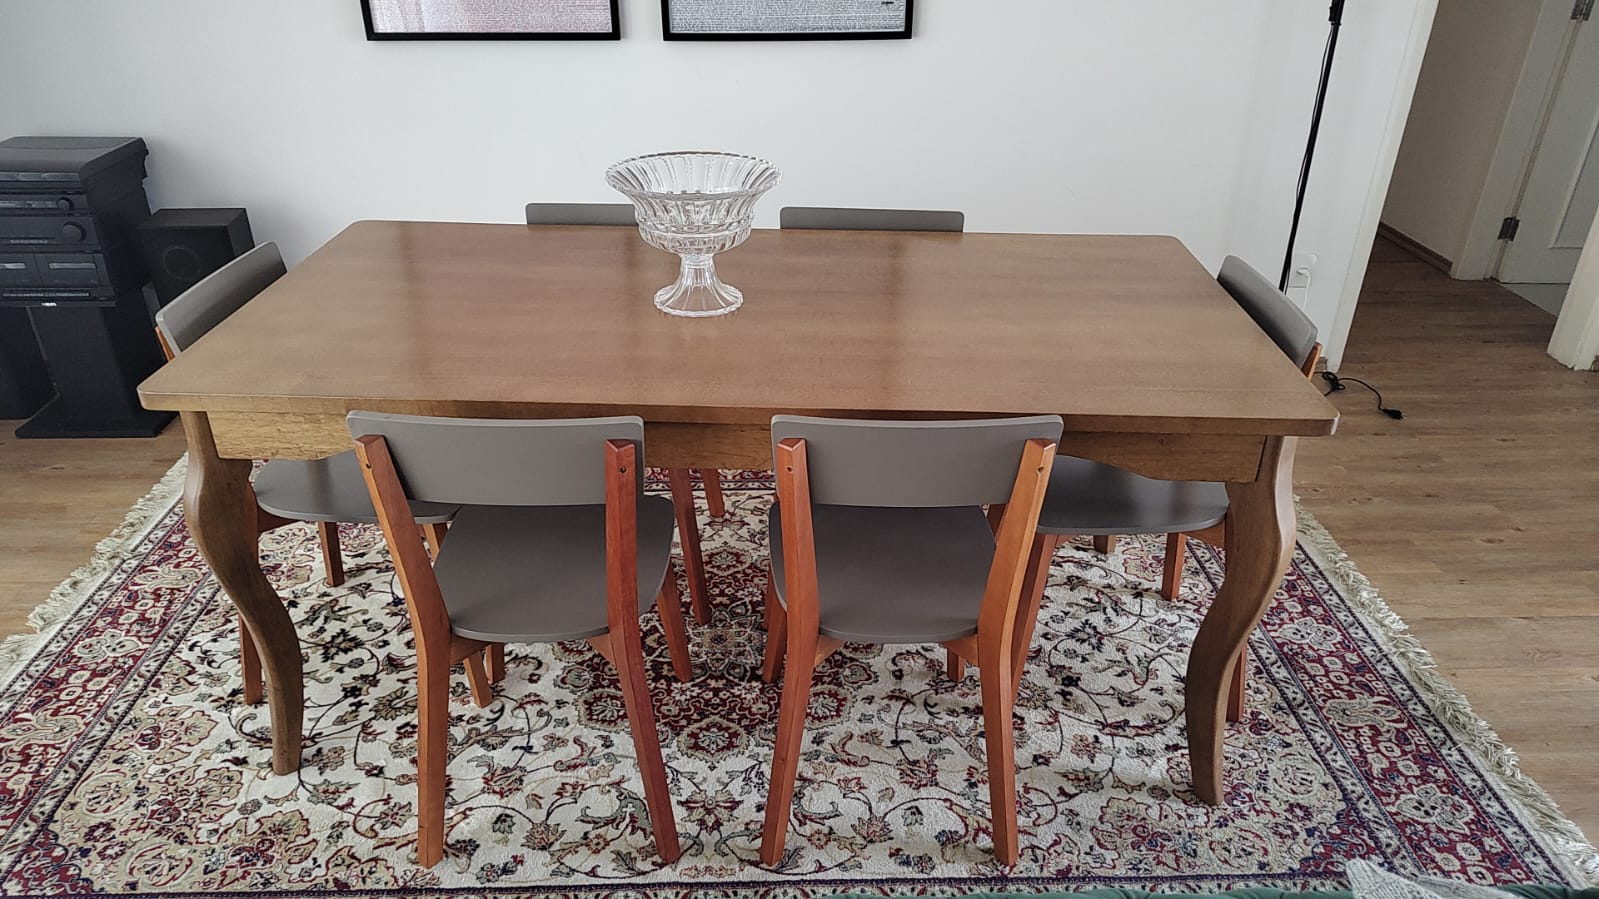
\includegraphics[width=\textwidth]{./MEDIA/MESA_JANTAR.jpeg}
\caption{Mesa de jantar Luís \textsc{xv} com seis cadeiras.}
\end{figure}
\noindent\textsc{\textbf{medidas}}
\begin{itemize}
\item Largura: 180\,cm (\textit{aproximado})
\item Altura: 100\,cm (\textit{aproximado})
\end{itemize}
\noindent\textsc{\textbf{valor}}
\begin{itemize}
\item \textsc{r}\$\,1\,900
\end{itemize}

\pagebreak

\begin{figure}[htpb!]
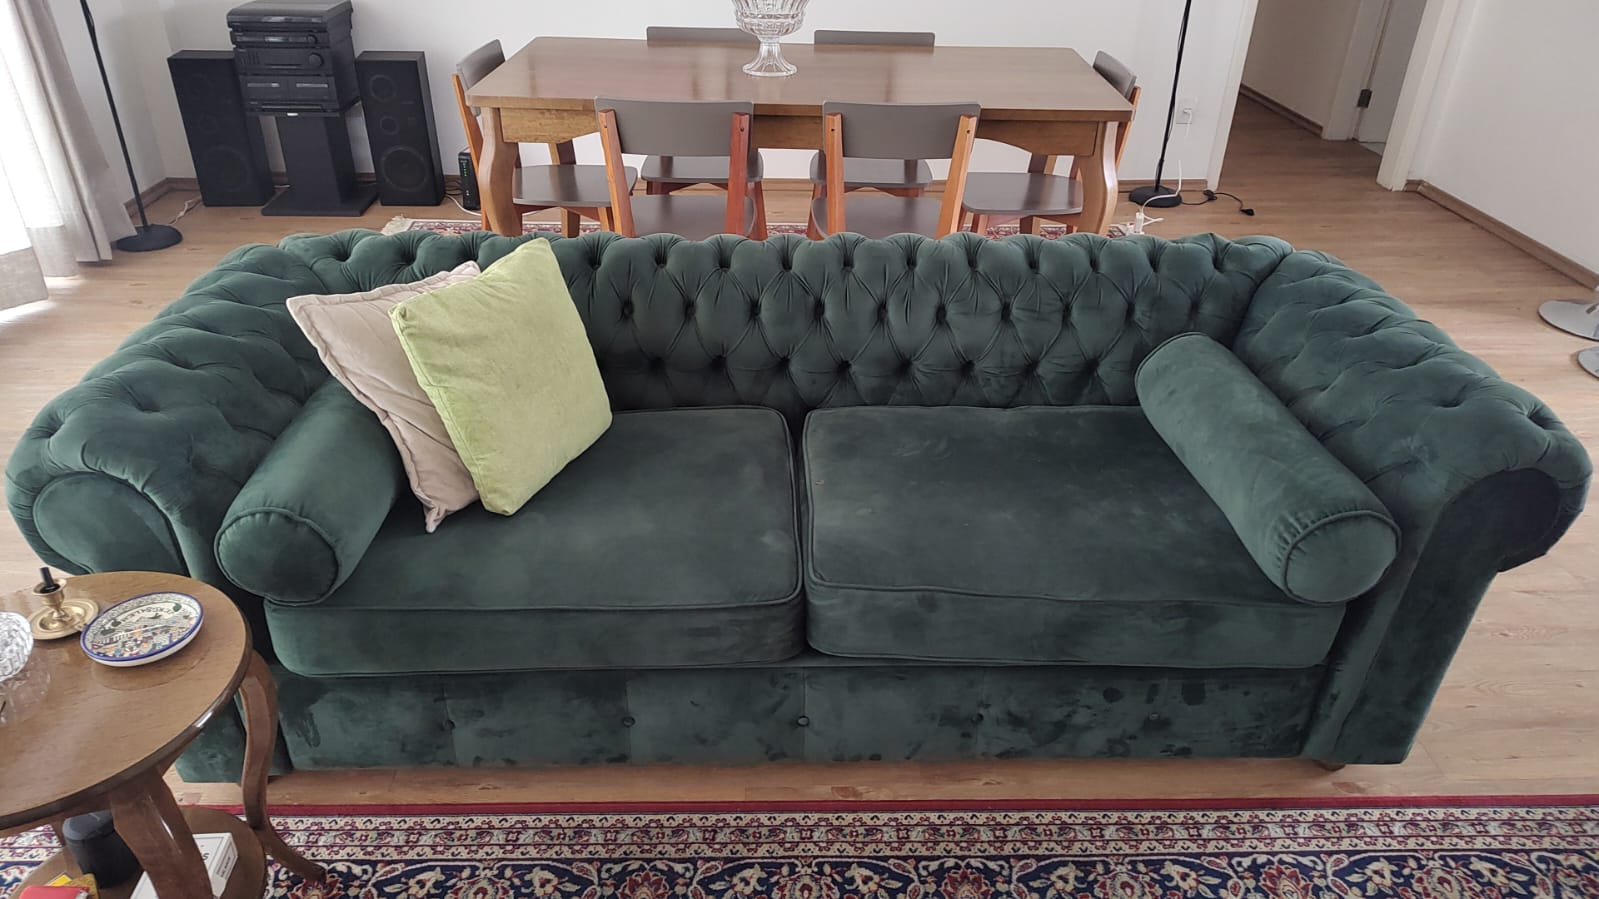
\includegraphics[width=\textwidth]{./MEDIA/SOFA.jpeg}
\caption{Sofá de veludo Chesterfield.}
\end{figure}
\noindent\textsc{\textbf{medidas}}
\begin{itemize}
\item Largura: 210\,cm (\textit{aproximado})
\item Altura: 100\,cm (\textit{aproximado})
\end{itemize}
\noindent\textsc{\textbf{valor}}
\begin{itemize}
\item \textsc{r}\$\,2\,400
\end{itemize}
\noindent\textsc{\textbf{observação}}
\begin{itemize}
\item Tem um defeito em uma das almofadas laterais, o zíper não fecha. Mas não é difícil de reparar.
\end{itemize}

\pagebreak

\begin{figure}[htpb!]
\begin{center}
\includegraphics[width=6cm]{./MEDIA/FOGAO.jpeg}
\caption{Fogão Brastemp quatro bocas em inox.}
\end{center}
\end{figure}
\noindent\textsc{\textbf{medidas}}
\begin{itemize}
\item Largura: 50\,cm
\item Altura: 85\,cm
\end{itemize}
\noindent\textsc{\textbf{valor}}
\begin{itemize}
\item \textsc{r}\$\,800
\end{itemize}
 
\pagebreak

\begin{figure}[htpb!]
\includegraphics[width=\textwidth]{./MEDIA/BOX.jpeg}
\caption{Baú box de veludo cereja.}
\end{figure}
\noindent\textsc{\textbf{medidas}}
\begin{itemize}
\item Comprimento: 55\,cm
\item Largura: 140\,cm
\item Altura: 40\,cm
\end{itemize}
\noindent\textsc{\textbf{valor}}
\begin{itemize}
\item \textsc{r}\$\,570
\end{itemize}

\pagebreak

\begin{figure}[htpb!]
\includegraphics[width=\textwidth]{./MEDIA/DIVA.jpeg}
\caption{Divã de veludo cereja.}
\end{figure}
\noindent\textsc{\textbf{medidas}}
\begin{itemize}
\item Comprimento: 70\,cm
\item Largura: 180\,cm
\item Altura: 90\,cm
\end{itemize}
\noindent\textsc{\textbf{valor}}
\begin{itemize}
\item \textsc{r}\$\,2\,200
\end{itemize}

\pagebreak

\begin{figure}[htpb!]
\includegraphics[width=\textwidth]{./MEDIA/MESINHA_PALITO.jpeg}
\caption{Mesinha de centro pé de palito.}
\end{figure}
\noindent\textsc{\textbf{medidas}}
\begin{itemize}
\item Largura: 90\,cm
\item Altura: 35\,cm
\end{itemize}
\noindent\textsc{\textbf{valor}}
\begin{itemize}
\item \textsc{r}\$\,400
\end{itemize}

\pagebreak

\begin{figure}[htpb!]
\includegraphics[width=\textwidth]{./MEDIA/MESINHA_CABECEIRA.jpeg}
\caption{Mesinha de cabeceira Luís \textsc{xv} off-white.}
\end{figure}
\noindent\textsc{\textbf{medidas}}
\begin{itemize}
\item Comprimento: 35\,cm
\item Largura: 55\,cm
\item Altura: 70\,cm
\end{itemize}
\noindent\textsc{\textbf{valor}}
\begin{itemize}
\item \textsc{r}\$\,500
\end{itemize}

\pagebreak

\begin{figure}[htpb!]
\begin{center}
\includegraphics[width=6cm]{./MEDIA/MESINHA_LATERAL.jpeg}
\caption{Mesinha lateral branca com tampo de madeira.}
\end{center}
\end{figure}
\noindent\textsc{\textbf{medidas}}
\begin{itemize}
\item Largura: 60\,cm
\item Altura: 72\,cm
\end{itemize}
\noindent\textsc{\textbf{valor}}
\begin{itemize}
\item \textsc{r}\$\,750
\end{itemize}

\pagebreak

\begin{figure}[htpb!]
\begin{center}
\includegraphics[width=6cm]{./MEDIA/CADEIRA.jpeg}
\caption{Cadeira de veludo verde musgo.}
\end{center}
\end{figure}
\noindent\textsc{\textbf{medidas}}
\begin{itemize}
\item Largura: 120\,cm (\textit{aproximadamente})
\item Altura: 70\,cm (\textit{aproximadamente})
\end{itemize}
\noindent\textsc{\textbf{valor}}
\begin{itemize}
\item \textsc{r}\$\,400
\end{itemize}

\pagebreak

\begin{figure}[htpb!]
\includegraphics[width=\textwidth]{./MEDIA/BANQUETAS.jpeg}
\caption{Duas banquetas.}
\end{figure}
\noindent\textsc{\textbf{medidas (cada uma)}}
\begin{itemize}
\item Largura: 50\,cm
\item Altura: 85\,cm
\end{itemize}
\noindent\textsc{\textbf{valor}}
\begin{itemize}
\item \textsc{r}\$\,500 (\textit{o par})
\end{itemize}
\noindent\textsc{\textbf{observações}}
\begin{itemize}
\item Tem marcas de falta de tinta na parte de trás dos assentos, conforme visível em foto. Mas não compromete o móvel.
\end{itemize}

\pagebreak

\begin{figure}[htpb!]
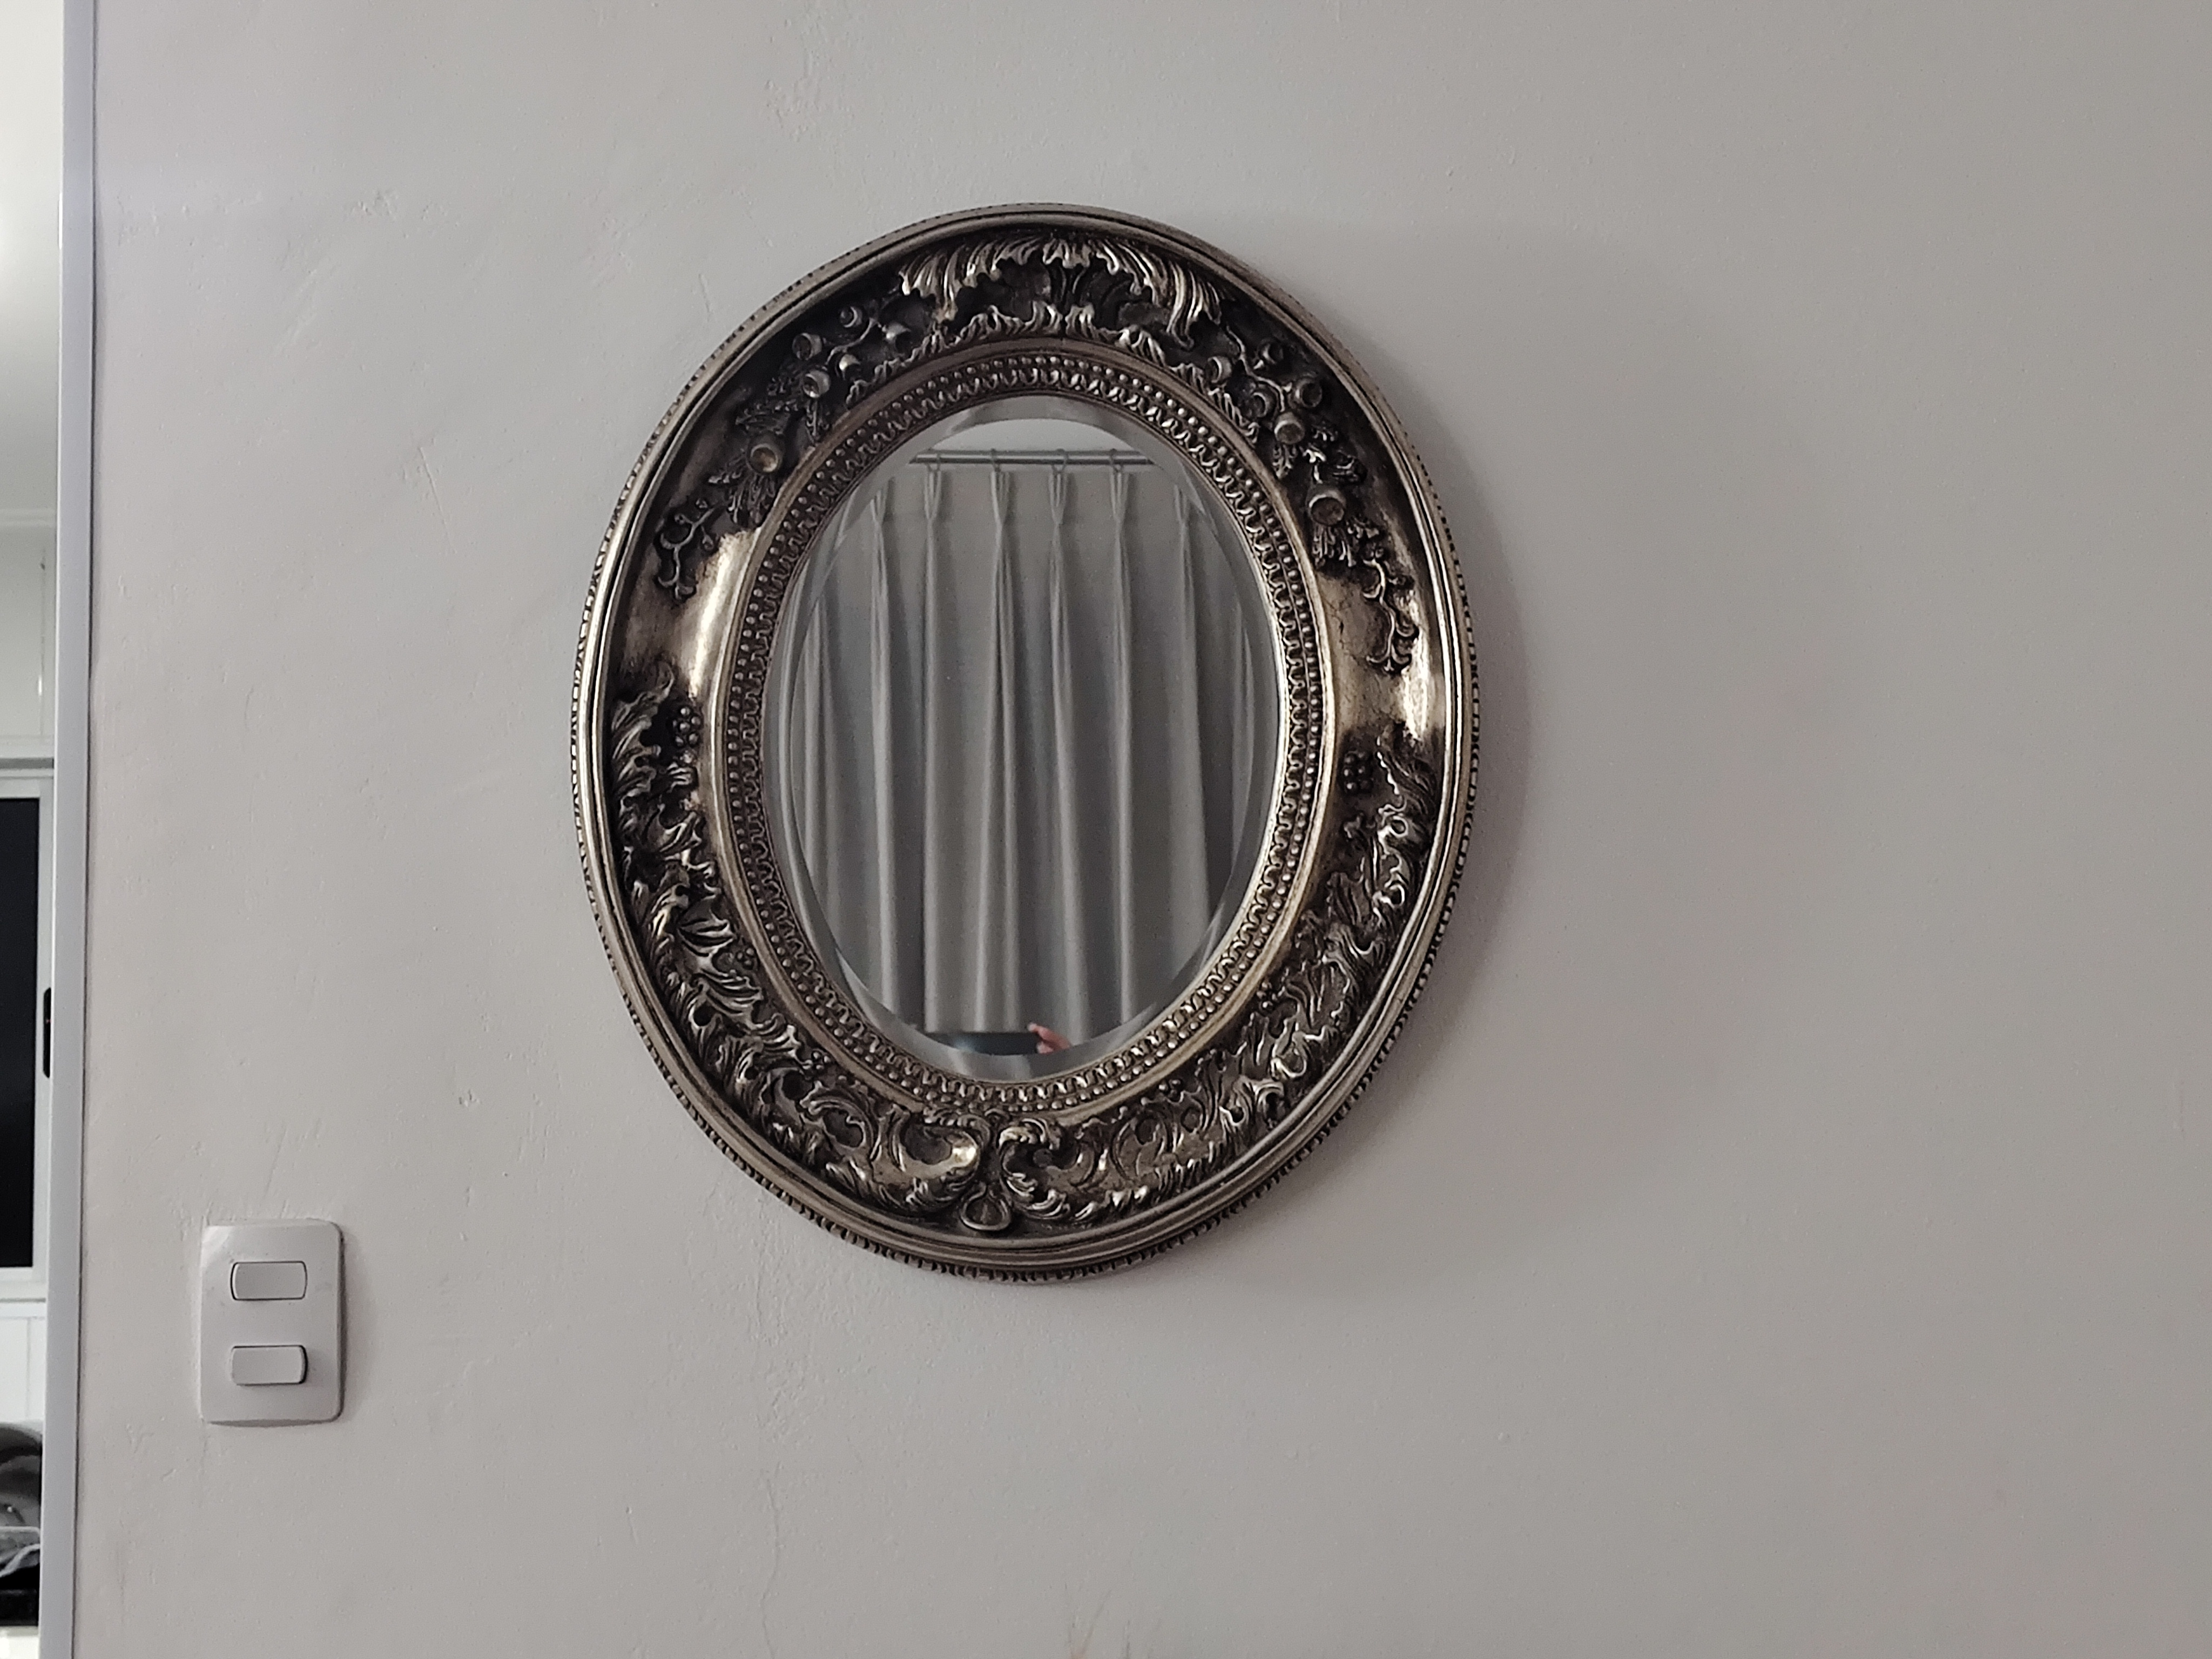
\includegraphics[width=\textwidth]{./MEDIA/ESPELHO_PEQUENO.jpeg}
\caption{Espelho dourado de rosto.}
\end{figure}
\noindent\textsc{\textbf{medidas}}
\begin{itemize}
\item Largura: 50\,cm
\item Altura: 60\,cm
\end{itemize}
\noindent\textsc{\textbf{valor}}
\begin{itemize}
\item \textsc{r}\$\,450
\end{itemize}

\pagebreak

\begin{figure}[htpb!]
\begin{center}
\includegraphics[width=6cm]{./MEDIA/ESPELHO_GRANDE.jpeg}
\caption{Espelho de corpo inteiro com moldura trabalhada em dourado.}
\end{center}
\end{figure}
\noindent\textsc{\textbf{medidas}}
\begin{itemize}
\item Largura: 70\,cm
\item Altura: 165\,cm
\end{itemize}
\noindent\textsc{\textbf{valor}}
\begin{itemize}
\item \textsc{r}\$\,800
\end{itemize}

\pagebreak

\mbox{}

\vfill

\noindent\textsc{\textbf{contato}}

\begin{itemize}
\item Responsável: Suzana Salama
\item E-mail: suzana@hedra.com.br
\item Telefone/\,WhatsApp: (11) 94534-7000
\end{itemize}

\endgroup
\pagebreak